\clearpage
\section{Developed work}
\label{ch:developed}

Esta seção apresenta o trabalho realizado até o momento que auxilia o desenvolvimento 
deste projeto de pesquisa de doutorado. 

This section presents the work carried out so far that is assisting the
development of this doctoral research project. \autoref{sec:module} talks about
some available software tools for performance evaluation and presents the new
OpenFlow module for simulations. \autoref{sec:scenario} introduces the proposed
\ac{SDN}-enabled \ac{LTE} simulation scenario, describing its design targets
and the network topology. Finally, \autoref{sec:controller} describes the
enhanced OpenFlow controller for the \ac{SDN}-enabled \ac{LTE} network.
% The work presented here is potential precursor of this doctoral research
% project.


%-----------------------------------------------------------------------------%
\subsubsection{Comparison between the developed works}
\label{subsec:applications}

In this part, we provide a feature comparison between various state-of-the-art bitrate
adaptation schemes in each category from the taxonomy in Figure 3.1. Table 3.1 summarizes
this comparison for each surveyed paper in terms of the following aspects:

\TODO{Montar tabela com trablhos relevantes}

Zhang et al. [5] focuses on the client-side, performing the average bitrate level by the bitrate
adaptation algorithm and the influence of chunk size variation for improve the QoE, while Shen et
al. [6] works with a set of cache proxy services to analyze the cache miss occurrences. This
work implements a reactive approach where cache proxies download the chunks of multimedia
content when requested. Rosário et al. [7] describes a multi-tier environment that provides a live
migration service from the cloud to the different tiers. The experimental scenarios delivery a
video stream between different tiers with QoE support. Poliakov et al. [3] deploy a DASH video
streaming with multiple sources. The DASH-client player can download the chunks, at the same
time, through different connections on the cloud. Archer et al. [8] proposes an algorithm to deal
with the cache replicas for flash bandwidth video provisioning, which is a critical bottleneck.

The aforementioned approaches could decrease the traffic load and improve QoE, but more
issues arise in Smart City scenarios: user mobility, collaborative cache schemes over multi-edge,
the amount of users during flash crowds, and interactive streaming requirements are not fully
considered. In this project we aim to design a video delivery system that considers such issues
to improve quality of experience for a range of video streaming needs, including low latency
requirements.

%-----------------------------------------------------------------------------%
\subsubsection{QoS-aware scheduling of tasks in fog computing}
\label{subsec:applications}




\ac{LTE} and WiFi mobile networks are focused on multimedia
applications over \ac{IP}. To provide a more realistic scenario for
simulations, four different multimedia streamings were adapted from
existing \ac{ns-3} applications, and are available for use during simulations:
\begin{itemize}
  \item An \emph{\ac{HTTP} application} simulates a client who establishes a
  \ac{TCP} connection with the server and sends a request for the main object
  of a given web page. When the client gets the main object, it process the
  message and start to request the inline objects of the given web page. After
  receiving all inline objects, the client waits a reading time interval before
  requesting a new main object of a new web page. This application was adapted
  from contributions sent to the ns-3-users mailing list, and the traffic model
  used in this application is based on the distributions indicated by
  \citet{Pries2012}.

  \item A \emph{Live Video Streaming application} simulates a unidirectional
  \ac{UDP} streaming following one trace among a collection of \acs{MPEG}-4
  video trace files presented by~\citet{Fitzek2001}. The average bit rate for a
  trace varies from 100\,Kbps to 1.1\,Mbps, and the file is randomly selected
  by the application. The average video length is expected to be 90
  seconds~\cite{youtubeStats} and is set by a normal distribution \ac{RNG}
  $\mathcal{N}(90,225)$. This application was adapted from the
  \texttt{UdpTraceFile} \ac{ns-3} application.

  \item A \emph{Buffered Video Streaming application} simulates a
  unidirectional \ac{TCP} video streaming, using the same traces from the live
  video streaming application, except that it can buffer the video and send it
  as fast as the network can support. The average video size is calculated to
  match the expected video length for the live streaming application. This
  application is based on the \texttt{BulkSendApplication} and
  \texttt{UdpTraceFile} \ac{ns-3} applications.
\end{itemize}

These four applications are used to provide five different types of traffic
flows in the network, with different \ac{QoS} requirements.
\autoref{tab:applications} shows the \ac{EPS} bearer mapping used for available
applications. Note that the traffic from the live video streaming application
can be sent over \ac{GBR} and Non-\ac{GBR} bearers.

\begin{table}[b!]
  \caption{Bearer \acs{QCI} mapping for applications.}
  \label{tab:applications}
  \centering
  \begin{tabular}{lll}
    \toprule
    \bfseries \acs{QCI} & \bfseries Bearer type & \bfseries Application \\
    \midrule
    1 & \ac{GBR}     & \ac{VoIP} \\
    2 & \ac{GBR}     & Live video streaming \\
    6 & Non-\ac{GBR} & Buffered video streaming \\
    7 & Non-\ac{GBR} & Live video streaming \\
    8 & Non-\ac{GBR} & \ac{HTTP} \\
    \bottomrule
  \end{tabular}
\end{table}

Apart from the established default bearer, any \ac{UE} can request for randomly
dedicated bearer context activations, observing the \ac{QCI} mapping in
\autoref{tab:applications}. Note that multiple bearers can be simultaneously
established with different \ac{QCI} values for a unique \ac{UE}. The individual
bearer requests generated by each \ac{UE} follows a \emph{Poisson Process} with
rate $\lambda = 0.\bar{3}$ requests per minute while the traffic length is
determined by the application. In this approach, the more active users on the
network, the greater is the aggregated Poisson process rate.

%-----------------------------------------------------------------------------%
\subsubsection{Network design and topology}
\label{subsec:design}

Instead of dismantling the \ac{LTE} network architecture, the currently
proposed scenario focus on the use of OpenFlow technology at the backhaul
network, connecting all \acp{eNB} and \acp{S-GW} via OpenFlow switches. The
backhaul network is responsible for carrying all the traffic for S1 and X2
interfaces, which is encapsulated withing the \ac{GTP}/\ac{UDP}/\ac{IP}
protocols. Considering the traffic routing and backward compatibility
challenges discussed in \autoref{subsec:challenges}, the proposed scenario
currently preserves the \ac{GTP} tunnels, so no \ac{EPS} element that handle S1
and X2 tunnel endpoints needs to be replaced and no changes in control
protocols are necessary. This approach allows a soft integration of new
OpenFlow network elements within a legacy infrastructure, with the help of
software controller.

Considering the \ac{GTP} protocol, some type of extension is necessary so the
OpenFlow switch can handle this tunneled traffic. Two options were examined:
the first was to improve the OpenFlow switch with virtual ports to remove
tunnel headers when the packet enters the switch and reconstruct it before
leaving; while the second option was to extend the OpenFlow switch and protocol
with new \ac{GTP} match fields. The former allows fine-grained matches in
packet payload but incurs in more processing power at switches to handle all
packet manipulations. The latter is simpler due to no de/encapsulation
operations, but can only match fields at tunnel headers (the outermost \ac{IP}
and \ac{UDP} headers). Even though, this second approach was preferred,
considering that tunnel headers also provide the necessary information that is
used for routing operations and \ac{QoS} provisioning. Also, the OpenFlow
protocol allows some type of header manipulation that can be used to bring
relevant information from encapsulated payload to outer headers. The new
OpenFlow \ac{OXM} match fields for \ac{GTP} protocol are specified under the
\ac{OXM} experimenter class, based on the work of \citet{Kempf2012a}. Two
fields are introduced: the 2 byte \ac{GTP} header flags field and the 4 byte
\ac{GTP} \ac{TEID} field.

Considering the network topology, \autoref{fig:epcof-scenario} shows the wired
portion for the simulation scenario. The backhaul network is a ring with an
arbitrary number of OpenFlow switches. A unified
\ac{S-GW}/\ac{P-GW}\footnote{This unified gateway approach is necessary due to
\ac{LENA} implementation restrictions in \ac{ns-3}.} gateway element is
attached to the first switch, and each other switch can have one or more
\acp{eNB} connected to it. Connections between OpenFlow switches are built with
Ethernet full duplex links, with configurable data rate and average delay
estimated at $100\,\mu$s, for a typical 20\,Km metropolitan fiber cable.

\begin{figure}[htb]
  \centering
    \subfloat[Wired backhaul network topology.]
    {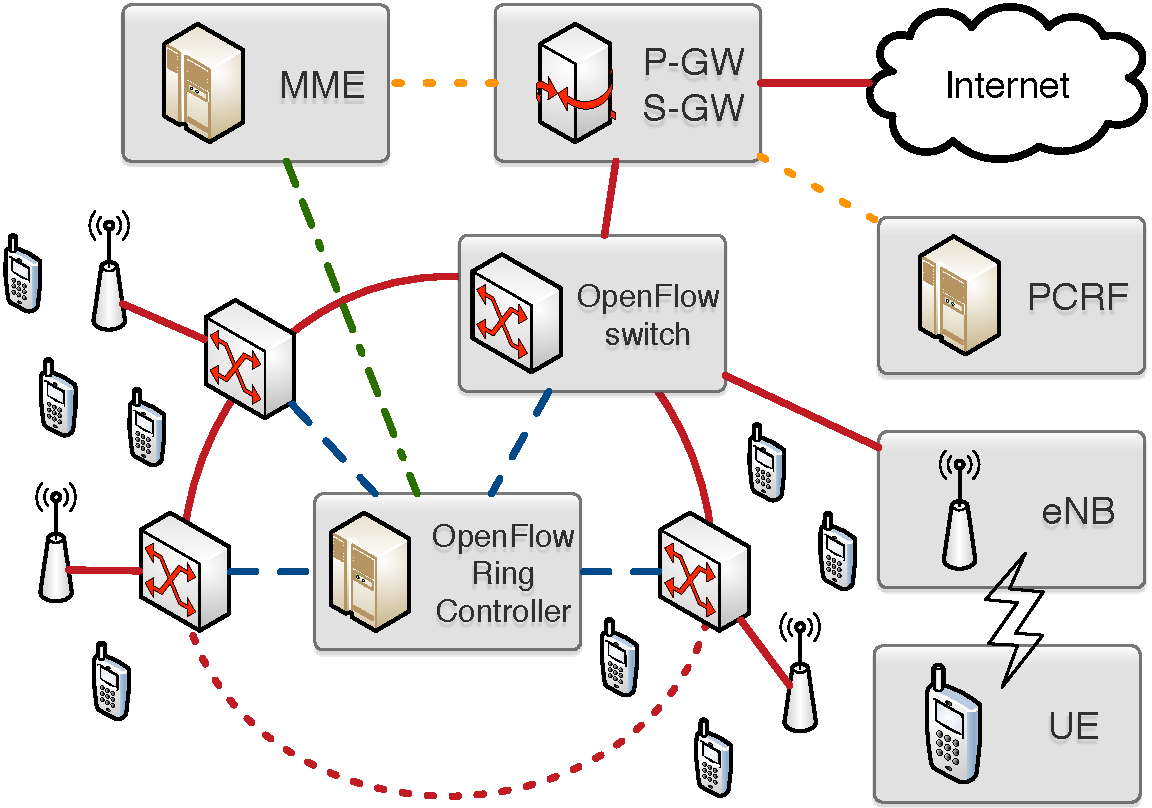
\includegraphics[width=.53\textwidth]{epcof-scenario}
    \label{fig:epcof-scenario}}
  \hfil \hspace{1cm}
    \subfloat[\acs{RAN} network topology.]
    {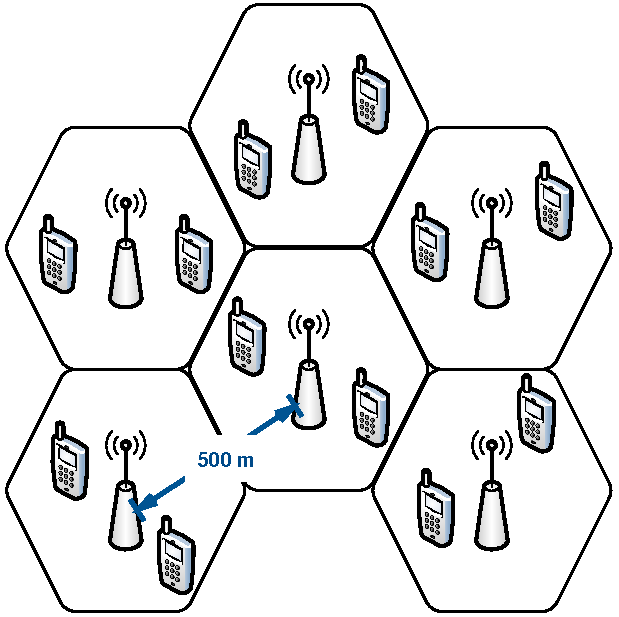
\includegraphics[width=.38\textwidth]{lte-scenario}
    \label{fig:lte-scenario}}
  \caption{\acs{SDN}-enabled \acs{LTE} network topology.}
  \label{fig:topology}
\end{figure}

Following the studies from \citet{Chundury2008} and \citet{Howard2011}, the
OpenFlow backhaul network is built over Ethernet technology, which is seen as
the most effective method to transport \ac{IP} packets and is the default
technology choice for a lower cost-per-bit as network scales to support large
capacity growth. The ring topology for backhaul network was chosen as most of
the legacy backhaul networks have a hub-spoke or ring access architecture.
Also, \citet{Nadiv2010} estate that the ring is one of the most efficient
topologies in terms of protection and is less costly than other topologies.
Nonetheless, it is possible to simulate different network topologies replacing
the connections between the switches.

\autoref{fig:lte-scenario} shows the \ac{RAN} topology, where each \ac{eNB}
covers an arbitrary number of active \acp{UE}. The \acp{eNB} are placed on a
hexagonal grid, 30 meters above the ground, and with an inter-site distance of
500 meters. \acp{UE} attached to each \ac{eNB} are scattered close to it, at
1.5 meters above the ground. \autoref{tab:lte-parameters} summarizes some of
the \ac{LENA} parameters that were adjusted in simulations. Any other \ac{LENA}
parameter not listed in the table was left on its default value.
